\documentclass{article}
\usepackage[utf8]{inputenc}

\title{Exercise 3}
\author{NTNU}
\date{TDT4165 fall 2018}

\usepackage{natbib}
\usepackage{graphicx}
\usepackage{listings}
\usepackage{color}
\usepackage{hyperref}
\definecolor{dkgreen}{rgb}{0,0.6,0}
\definecolor{gray}{rgb}{0.5,0.5,0.5}
\definecolor{mauve}{rgb}{0.58,0,0.82}

\lstset{frame=tb,
  language=Haskell,
  aboveskip=3mm,
  belowskip=3mm,
  showstringspaces=false,
  columns=fixed,
  basicstyle={\small\ttfamily},
  numbers=none,
  numberstyle=\tiny\color{gray},
  keywordstyle=\color{blue},
  commentstyle=\color{dkgreen},
  stringstyle=\color{mauve},
  breaklines=true,
  breakatwhitespace=true,
  tabsize=3,
  numbers=left,
  stepnumber=1
}

\begin{document}

\maketitle

\section{The power of types: Hoogle}
\subsection{Type inference}
The type system in Haskell is quite powerful, as you might have discovered. Even if we do not include a type signature, we can ask GHC to tell us its type and get an answer. This is called \textbf{type inference}.
\lstset{language=Haskell}
\begin{lstlisting}
Prelude> import Data.Char
Prelude Data.Char> :t ord
ord :: Char -> Int
Prelude Data.Char> let fun = map ord
Prelude Data.Char> :t fun 
fun :: [Char] -> [Int]
\end{lstlisting}
GHC infers the type of the function \textbf{fun} from the function \textbf{ord} that is passed to map. Since map has type \textbf{(a $\rightarrow$ b) $\rightarrow$ [a] $\rightarrow$ [b]}, and ord has type \textbf{Char $\rightarrow$ Int}, \textbf{map ord must have type [Char] $\rightarrow$ [Int]}.\\
For the curious, a description of a type inference algorithm can be found here (not curriculum): \url{http://www.cs.tau.ac.il/~msagiv/courses/pl14/chap6-1.pdf}

\textcolor{dkgreen}{\subsection{Hoogle}
A consequence of the type system and type inference, is that it is possible to create a database where you can \textcolor{black}{\textbf{search for functions based on their arguments and return types}}. It is not only possible, it exists!\\
At \textcolor{mauve}{\url{https://www.haskell.org/hoogle/}}, you can search through standard libraries using type signature, function name, type name and much, much more. You can also search for keywords.}
Clicking on the name of the type class or function, then on #Source, will bring you to its declaration in source.\\
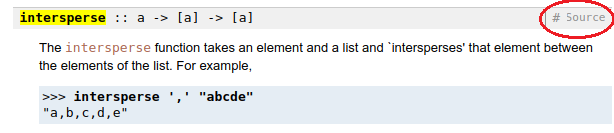
\includegraphics[scale=0.5]{hoogle.png}

\section{Bounded parametric polymorphism}
Last week, we saw functions like \textbf{id :: a $\rightarrow$ a} that are polymorphic across \emph{all} types, but we've also seen functions like \textbf{show :: Show a $\Rightarrow$ a $\rightarrow$ String} that are polymorphic across all types that are "showable". Here \textbf{Show} is a \emph{type class}, and any type belonging to \textbf{Show} must implement the function \textbf{show}.

\subsection{Type classes and instances}
Let us define a function and ask GHC to tell us what types we are dealing with:
\lstset{language=Haskell}
\begin{lstlisting}
eq x y
    | x == y    = x
    | otherwise = y
    
> :t eq
> eq :: Eq a => a -> a -> a
\end{lstlisting}
 The \textbf{Eq} type class simply allows checking if two elements are equal or not:
\begin{lstlisting}
class Eq a where
  (==) :: a -> a -> Bool
  (/=) :: a -> a -> Bool
  
  x == y = not (x /= y)
  x /= y = not (x == y)
\end{lstlisting}
The last two lines give default implementations of equality (\textbf{==}) in terms of inequality (\textbf{/=}), and vice versa. This means a \emph{minimal complete definition} of \textbf{Eq} requires only one of them. For primitive types such as Int, the \textbf{Eq} instance is has a low-level implementation. However, for types we have declared ourselves, we may need to implement the instance ourselves. Consider the type constructor \textbf{Maybe} defined in exercise 2. We would like \textbf{Maybe a} to inherit equality from \textbf{a}, meaning that \textbf{Just x} equals \textbf{Just y} if and only if \textbf{x} equals \textbf{y}:
\begin{lstlisting}
data Maybe a = Just a | Nothing

instance Eq a => Eq (Maybe a) where
    Nothing == Nothing   = True
    (Just x) == (Just y) = x == y
    _ == _               = False
\end{lstlisting}
The case of inheriting a type class is very common, and there is a shorthand to avoid writing out the instance explicitly, namely by \emph{deriving}:
\begin{lstlisting}
data Maybe a = Just a | Nothing deriving Eq
\end{lstlisting}

\subsection{List functions}
Implement the functions \textbf{listSum}, \textbf{listProduct}, \textbf{listConcat}, \textbf{listMaximum} and \textbf{listMinimum}, that sums a list, takes the product of a list, concats a list of lists, finds the largest and smallest element in a list, respectively. \textbf{Use pattern matching on list and recursion.} Some useful pattern matching syntax:
\begin{lstlisting}
-- [] matches an empty list
example [] = ...
-- here, lst refers to the whole list, x refers to the first element, and xs refers to the tail of the list
example lst@(x:xs) = ...
\end{lstlisting}

\section{More higher-order functions: folds}

The functions you implemented in task 2, are all ways of reducing a list to a single value, and if you were implementing these as a for-loop you'd have a single state that you'd update on each iteration. This pattern of iteration is captured by a \emph{fold}. Now, lists can be iterated over either from the top or from the bottom (or left to right if you prefer). Laziness makes it more efficient to iterate from the right (ask us about this!), and we'll therefore have a look at \textbf{foldr}:
\begin{lstlisting}
foldr :: (a -> b -> b) -> b -> [a] -> b
foldr op acc xs = ... 

foldr (+) 0 [1,2,3] -- example of a step-wise reduction
==> 1 + (foldr (+) 0 [2,3])
==> 1 + (2 + (foldr (+) 0 [3]))
==> 1 + (2 + (3 + 0))
==> 1 + (2 + 3)
==> 1 + 5
==> 6
\end{lstlisting}
By how our lists are defined, the head is always what we see first. What makes foldr "folding from the right" is how the actual addition is being done. In the above example, the first addition performed is "3 + 0". The variable \texttt{acc} is the \emph{accumulator} and is the state if you were to do a for-loop. 

\subsection{Foldable}
Lists aren't the only data-structure that can be reduced to a single value, and we'll see how it can be done for (binary) trees in the next section. The underlying type class for things that are "foldable" is \textbf{Foldable}:
\begin{lstlisting}
class Foldable t where
  foldr :: (a -> b -> b) -> b -> t a -> b
\end{lstlisting}
It is an immediate generalization of \textbf{foldr} for lists, we've only replaced \texttt{[a]} by \texttt{t a} where \texttt{t} is another type constructor. To put this into perspective, remember that as a type constructor \texttt{[]} takes a type \texttt{a} and constructs the type \texttt{[a]} i.e. \emph{the lists with elements in \texttt{a}}. Likewise, \texttt{Maybe} takes any type \texttt{a} and constructs the type \texttt{Maybe a}. (Is Maybe foldable?) The \texttt{t} in our \textbf{Foldable} class is any such type constructor.

In this week's exercise you are asked to implement an instance of \textbf{Foldable} for lists, and to define a set of related functions.

\subsection{Binary trees}
The goal of this section is to understand how we may represent binary trees (called \texttt{Tree2} below) in Haskell and make our Tree type an instance of \textbf{Foldable}. Before reading on, try to define your own binary tree type, and please ask if you have no clue! (There are many ways, e.g. should the branches have values?)

First of all, a \emph{binary} tree is one where branches split into \emph{two}, and you could think of our representation of lists as "unary trees" (\texttt{Tree1} below) which only have one, continuous branch. With this analogy:
\begin{lstlisting}
data List a = Cons a (List a) | Nil -- same as a : [a] | []
data Tree1 a = Branch a (Tree1 a) | Leaf1 a
data Tree2 a = Branch (Tree2 a) a (Tree2 a) | Leaf a
\end{lstlisting}
Now, as with lists, we can make sense of summing all the values of a \textbf{Tree2}, or taking their product, maximum or minimum---even concatenating them makes sense. This should be an indication that \textbf{Tree2} can have a \textbf{Foldable} instance. As a hint, your implementation should produce the following reductions:
\begin{lstlisting}
foldr (+) 0 (Leaf 1)  ==> 1 + 0
foldr (+) 0 (Branch (Leaf 1) 2 (Leaf 3))
==> foldr (+) (2 + foldr (+) 0 (Leaf 3)) (Leaf 1)
==> 1 + (2 + foldr (+) 0 (Leaf 3))
==> 1 + (2 + (3 + 0)) ...
\end{lstlisting}
The skeleton for this task can be found in src/Tree.hs. Make the tree an instance of \textbf{Foldable}. Writing the three predefined functions might help you reason about this task, but they are not mandatory.

\section{The Num type class}
\subsection{Num Complex}
A Complex type is already defined in the source file. It is a member of the Show and Eq type classes. Make it an instance of the Num type class by implementing the functions below. This is the minimal complete definition of Num.
\lstset{language=Haskell}
\begin{lstlisting}
(+), (*) :: Num a => a -> a -> a
abs, signum :: Num a => a -> a
fromInteger :: Num a => Integer -> a
(-) :: Num a => a -> a -> a
or
negate :: Num a => a -> a
\end{lstlisting}
This is the minimal implementation of a type for it to be included in the Num type class. An explanation of the functions and rules for complex numbers, are outlined below.

\subsection{(+)}
Addition of two complex numbers.
\[(a+bi)+(c+di)=(a+c)+(b+d)i\]

\subsection{(*)}
Multiplication of two complex numbers.
\[(ac-bd) + (ad+bc)i\]

\subsection{abs}
Absolute value of a complex number.
\[|a+bi|=\sqrt{a^2+b^2}\]

\subsection{signum}
The sign of a complex number.
\[sign(z) = \frac{z}{|z|}\]

\subsection{fromInteger}
Conversion from an Integer to the complex representation of this integer. For a Double, \textbf{fromInteger 7} will return \textbf{7.0}.

\subsection{(negate $|$ (-))}
Implement either negate (unary minus), which returns the negation of the number it receives, \textbf{or} (-) that performs subtraction.
\[(a-bi)+(c-di)=(a-c)+(b-d)i\]

\section{Making your own type classes}

\subsection{Record syntax}
Using record syntax, we can create types with named fields.
\begin{lstlisting}
--record syntax
data Person = Person { firstName :: String
                     , lastName :: String
                     , socialSecNr :: Int
                     , zipCode :: Int
                     } deriving (Eq, Show)
\end{lstlisting}
Above, we have defined a type \textbf{Person}, using record syntax. The fields are easy to access.
\begin{lstlisting}
Prelude> let person1 = Person {firstName = "Jane", lastName = "Doe", socialSecNr = 1234567890, zipCode = 7034}
Prelude> firstName person1
"Jane"
\end{lstlisting}
The person type defined above, is a derived instance of Show and Eq. (==) will then result in a comparison of every field and False if they are not all equal. This is unfortunate, since Jane might move or change her name. To amend this, we write our own instance of Eq.
\begin{lstlisting}
instance Eq Person where
    (==) p1 p2 = socialSecNr p1 == socialSecNr p2
--now Jane can move all she wants and still be the same person
Prelude> let samePers = person1 {zipCode = 7042}
Prelude> samePers == person1
True
\end{lstlisting}
\subsection{Move type class}
Create a type class Move that is a subclass of Pos. A movable type should be able to be moved and has a position where it belongs.

\subsection{Car}
Create a type \textbf{Car}, using record syntax, and make it an instance of Eq, Pos and Move.

\subsection{Key}
Create a type \textbf{Key}, using record syntax, and make it an instance of Eq, Pos and Move.

\subsection{free}
Implement a function \textbf{free :: Move a $\Rightarrow$ a $\rightarrow$ Bool} that checks if an object is at the place it belongs.

\subsection{carAvailable}
Implement a function \textbf{carAvailable :: Car $\rightarrow$ Bool} that checks if the car and its keys are free.

\subsection{distanceBetween}
Implement a function \textbf{distanceBetween :: Pos a $\Rightarrow$ a $\rightarrow$ a $\rightarrow$ (Position or Int)} which calculates the distance between two positions. You are free to choose your own definition of \textit{distance}.

\section{Theory questions}
\begin{itemize}
    \item When implementing \textbf{treeMaximum} in src/Tree.hs, do you have to return a Maybe? Why or why not?
    \item After making \textbf{Tree a} an instance of \textbf{Foldable}, we can sum it by calling \textbf{sum \$ Branch (Leaf 56) 2 (Leaf 23)} (:l src/Tree.hs and try it out!). This also applies to \textbf{maximum} and several other functions. How do we get these functions "for free"?
    \item Can we make Complex an instance of Ord? The minimal complete definition of Ord is \textbf{compare | ($<$=)}, meaning that you have to implement either compare or ($<$=). Use Hoogle to inspect these functions in more detail, if needed. Provide the reasoning behind your answer.
    \item Load your file and write \textbf{negate (Complex 3 4)}, if you implemented (-) in 2.7. If you implemented negate, type \textbf{(Complex 3 4) - (Complex 2 7)}. What happens? Why does this happen?
    \item Try to make a Pos instance of the type synonym Position. What kind of error message do you get? From the error message, do you think it's possible to achieve this?
    \item You used record syntax when creating your types, and you might have run into issues if you tried to name fields identically. If not, try to run the following code:
    \lstset{language=Haskell}
    \begin{lstlisting}
data Employee = Employee { name :: String
                         , employeenr :: Int }
                         
data Student = Student { name :: String
                       , studentnr :: Int }
    \end{lstlisting}
    What kind of error message do you get? Why do you get this error message? Hint: Remove one of the entries, load the file and ask for the type of a field. What's the scope of the entry?
\end{itemize}

\end{document}
